\chapter{Reconstruction}
\label{chap:reconstruction}

Chapter \ref{chap:experiment} discusses how a proton-proton collision may be captured by a physical 
detector and turned into data that may be stored and analyzed. Chapter \ref{chap:simulation} discusses 
the simulation of this same process. At this most basic level, however, the ATLAS detector is only a machine 
for turning particles into a set of electrical signals, albeit in a very sophisticated, physics motivated way. 
This chapter discusses the step of turning these electrical signals into objects which may be identified 
with the underlying physics processes, and therefore used to make statements about what occured within 
a given collision event. This process is termed \emph{reconstruction}, and we will focus particularly on jets and flavor tagging, as the most relevant pieces for this thesis work.

\section{Jets}
As discussed in Chapters \ref{chap:experiment} and \ref{chap:simulation}, the production of particles with color 
charge from a proton-proton interaction is complicated both by parton showering and by confinement: a quark produced 
from a hard scatter is not seen as a quark, but rather, as a spray of particles with a variety of hadrons in the final 
state, which subsequently shower upon interaction with the calorimeter in a complicated way. 

For hard scatter electrons, photons, or muons on the other hand, the picture is much clearer: there is no parton 
showering, and each has a distinct signature in the detector: photons have no tracks and a very localized calorimeter
shower, electrons are associated with tracks and are similarly localized in the calorimeter, and muons are associated 
with tracks, pass through the calorimeter due to their large mass, and leave signatures in the muon spectrometer.

Jets are a tool to deal with the messiness of quarks and gluons. The basic concept is to group the multitude of
particles produced by a quark or gluon decay into a single object. Such an object then has associated properties, 
including a four-vector, which may be identified with the corresponding initial state particle. In practice a variety 
of information from the ATLAS detector is used for such a reconstruction. The analysis considered in this thesis uses 
particle flow jets~\cite{PERF-2015-09}, which combines information from both the tracker and the calorimeter, where the 
combined objects may be identified with underlying particles. However, jets built from clusters of calorimeter cells~\cite{PERF-2014-07} as well as from charged particle tracks~\cite{ATL-PHYS-PUB-2017-010} have also been used very effectively.

A variety of algorithms are used to associate detector level objects to a given jet. The most commonly used 
in ATLAS is the anti-$k_{T}$ algorithm~\cite{Antikt}, which is a successor to the $k_{T}$ algorithm, among others~\cite{Jetography}, and develops as follows. Both algorithms are sequential recombination algorithms, which begin with the smallest distance, $d_{ij}$ between considered objects (e.g. particles or intermediate groupings of particles). If $d_{ij}$
is less than a parameter $d_{iB}$ (B for ``beam'') object $i$ is combined with object $j$, the distance $d_{ij}$ is recomputed, and the process repeats. This proceeds until $d_{ij} \geq d_{iB}$, at which point the jet is ``complete''
and removed from the list of considered objects.

The definitional difference between $k_{T}$ and anti-$k_{T}$ is these distance parameters. In 
general form, these are defined as 
\begin{align}
d_{ij} &= \min(p_{Ti}^{2p},p_{Tj}^{2p})\frac{\Delta R_{ij}^2}{R^2}\\
d_{iB} &= p_{Ti}^{2p}
\end{align}
where $p_{Ti}$ is the transverse momentum of object $i$, $\Delta R_{ij}$ is the angular distance between 
objects $i$ and $j$, $R$ is a radius parameter, and $p$ controls the tradeoff between the $p_{T}$ and angular 
distance terms. For the $k_{T}$ algorithm $p=1$; for the anti-$k_{T}$ algorithm, $p=-1$. This is a simple 
change, but results in significantly different behavior. 

The anti-$k_{T}$ algorithm can be understood as follows: for a single high $p_{T}$ particle ($p_{T1}$) 
surrounded by a bunch of low $p_{T}$ particles, the low $p_{T}$ particles will be clustered with the high $p_{T}$ one if
\begin{align}
&d_{1j} = \frac{1}{p_{T1}^2}\frac{\Delta R_{1j}^2}{R^2} < \frac{1}{p_{T1}^2}\\
&\implies \Delta R_{1j} < R.
\end{align}
Therefore, a single high $p_{T}$ particle ($p_{T1}$) surrounded by a bunch of low $p_{T}$ particles results 
in a perfectly conical jet. This shape may change with the presence of other high momentum particles, but the
key feature of the dynamics is that the jet shape is determined by high $p_{T}$ objects due to the $\frac{1}{p_{T}}$
nature of this definition. In contrast, the $k_{T}$ algorithm results in jets influenced by low momentum particles, 
which results in a less regular shape. This property, of regular jet shapes determined by high momentum objects, 
as well as demonstrated good practical performance, makes the anti-$k_{T}$ algorithm the favored jet algorithm in ATLAS.

Because jets are composed of multiple objects, a useful property of jets is jet \emph{substructure}, that is, 
acknowledging that jets are composite objects, analyzing the structure of a given jet to infer physics information. 
This leads to the use of \emph{subjets}; that is, after running jet clustering, often to create a``large-R'', $R=1.0$ 
anti-$k_{T}$ jet, a smaller radius jet clustering algorithm is run within the jet. Subjets are often chosen using the 
$k_{T}$ algorithm, which again is sensitive to lower momentum particles, with $R=0.2$ or 0.3. For the boosted version 
of this thesis analysis, such a strategy is used, in which the subjets are \emph{variable radius} and depend on the 
momentum of the (proto)jet in question. Beyond this thesis work, substructure is used in a large variety of analyses, 
with a set of associated variables and tools developed for exploiting this structure \todo{Cite some?}.
 
\section{Flavor Tagging}
For this this thesis, the physics process being considered is $HH\rightarrow \bbbb$. From the previous section, we 
know that the standard practice is to identify these $b$ quarks (or, rather, the resulting $B$ hadrons, due to confinement) 
with jets -- in our case, these \emph{$b$-jets} are R=0.4 anti-$k_{T}$ particle flow jets (see Chapter \ref{chap:bbbb}). 
However, not all jets produced at the LHC are from $B$ hadrons; rather, there are a variety of different types of jets 
corresponding to different flavors of quarks. These are often classified as light jets (from $u$, $d$, or $s$ quarks, or 
gluons) or as other \emph{heavy flavor} jets, e.g. $c$-jets, involving $c$ quarks. Distinguishing between these different 
categories is a very active area of work in ATLAS, termed \emph{flavor tagging}, with much focus on \emph{$b$-tagging} in 
particular, that is, the identification of jets from $B$ hadron decays. We here briefly describe the techniques used 
for flavor tagging in ATLAS.

What distinguishes a $b$-jet from any other jet? This question is fundamental to the design of the various $b$-tagging 
algorithms, and has two major answers: (1) $B$ hadrons have long lifetimes, and (2) $B$ hadrons have large masses. 
It is most illustrative to compare the $B$ hadron properties to a common light meson, e.g. $\pi^{0}$, the neutral 
pion, with quark content $\frac{1}{\sqrt{2}}(u\bar{u}-d\bar{d})$. $B$ hadrons have lifetimes around \SI{1.5}{\ps},
corresponding to a decay length $c\tau\approx 0.45$mm. In contrast, $\pi^0$ has a lifetime of $8.4\times 10^{-5}$ps, 
which is around 20,000 times shorter! Theoretically, this comes from CKM suppresion of the $b$ to $c$ transition \todo{check}, which dominates the $B$ decay modes. Experimentally, this difference pops up as shown in 
Figure \ref{fig:bjet-diagram} -- light flavor initiated jets decay almost immediately at the proton-proton 
interaction point, whereas b-jets are distinguished by a displaced secondary vertex, corresponding to the 5 mm decay 
length calculated above.

\begin{figure}[ht]
\label{fig:bjet-diagram}
\centering
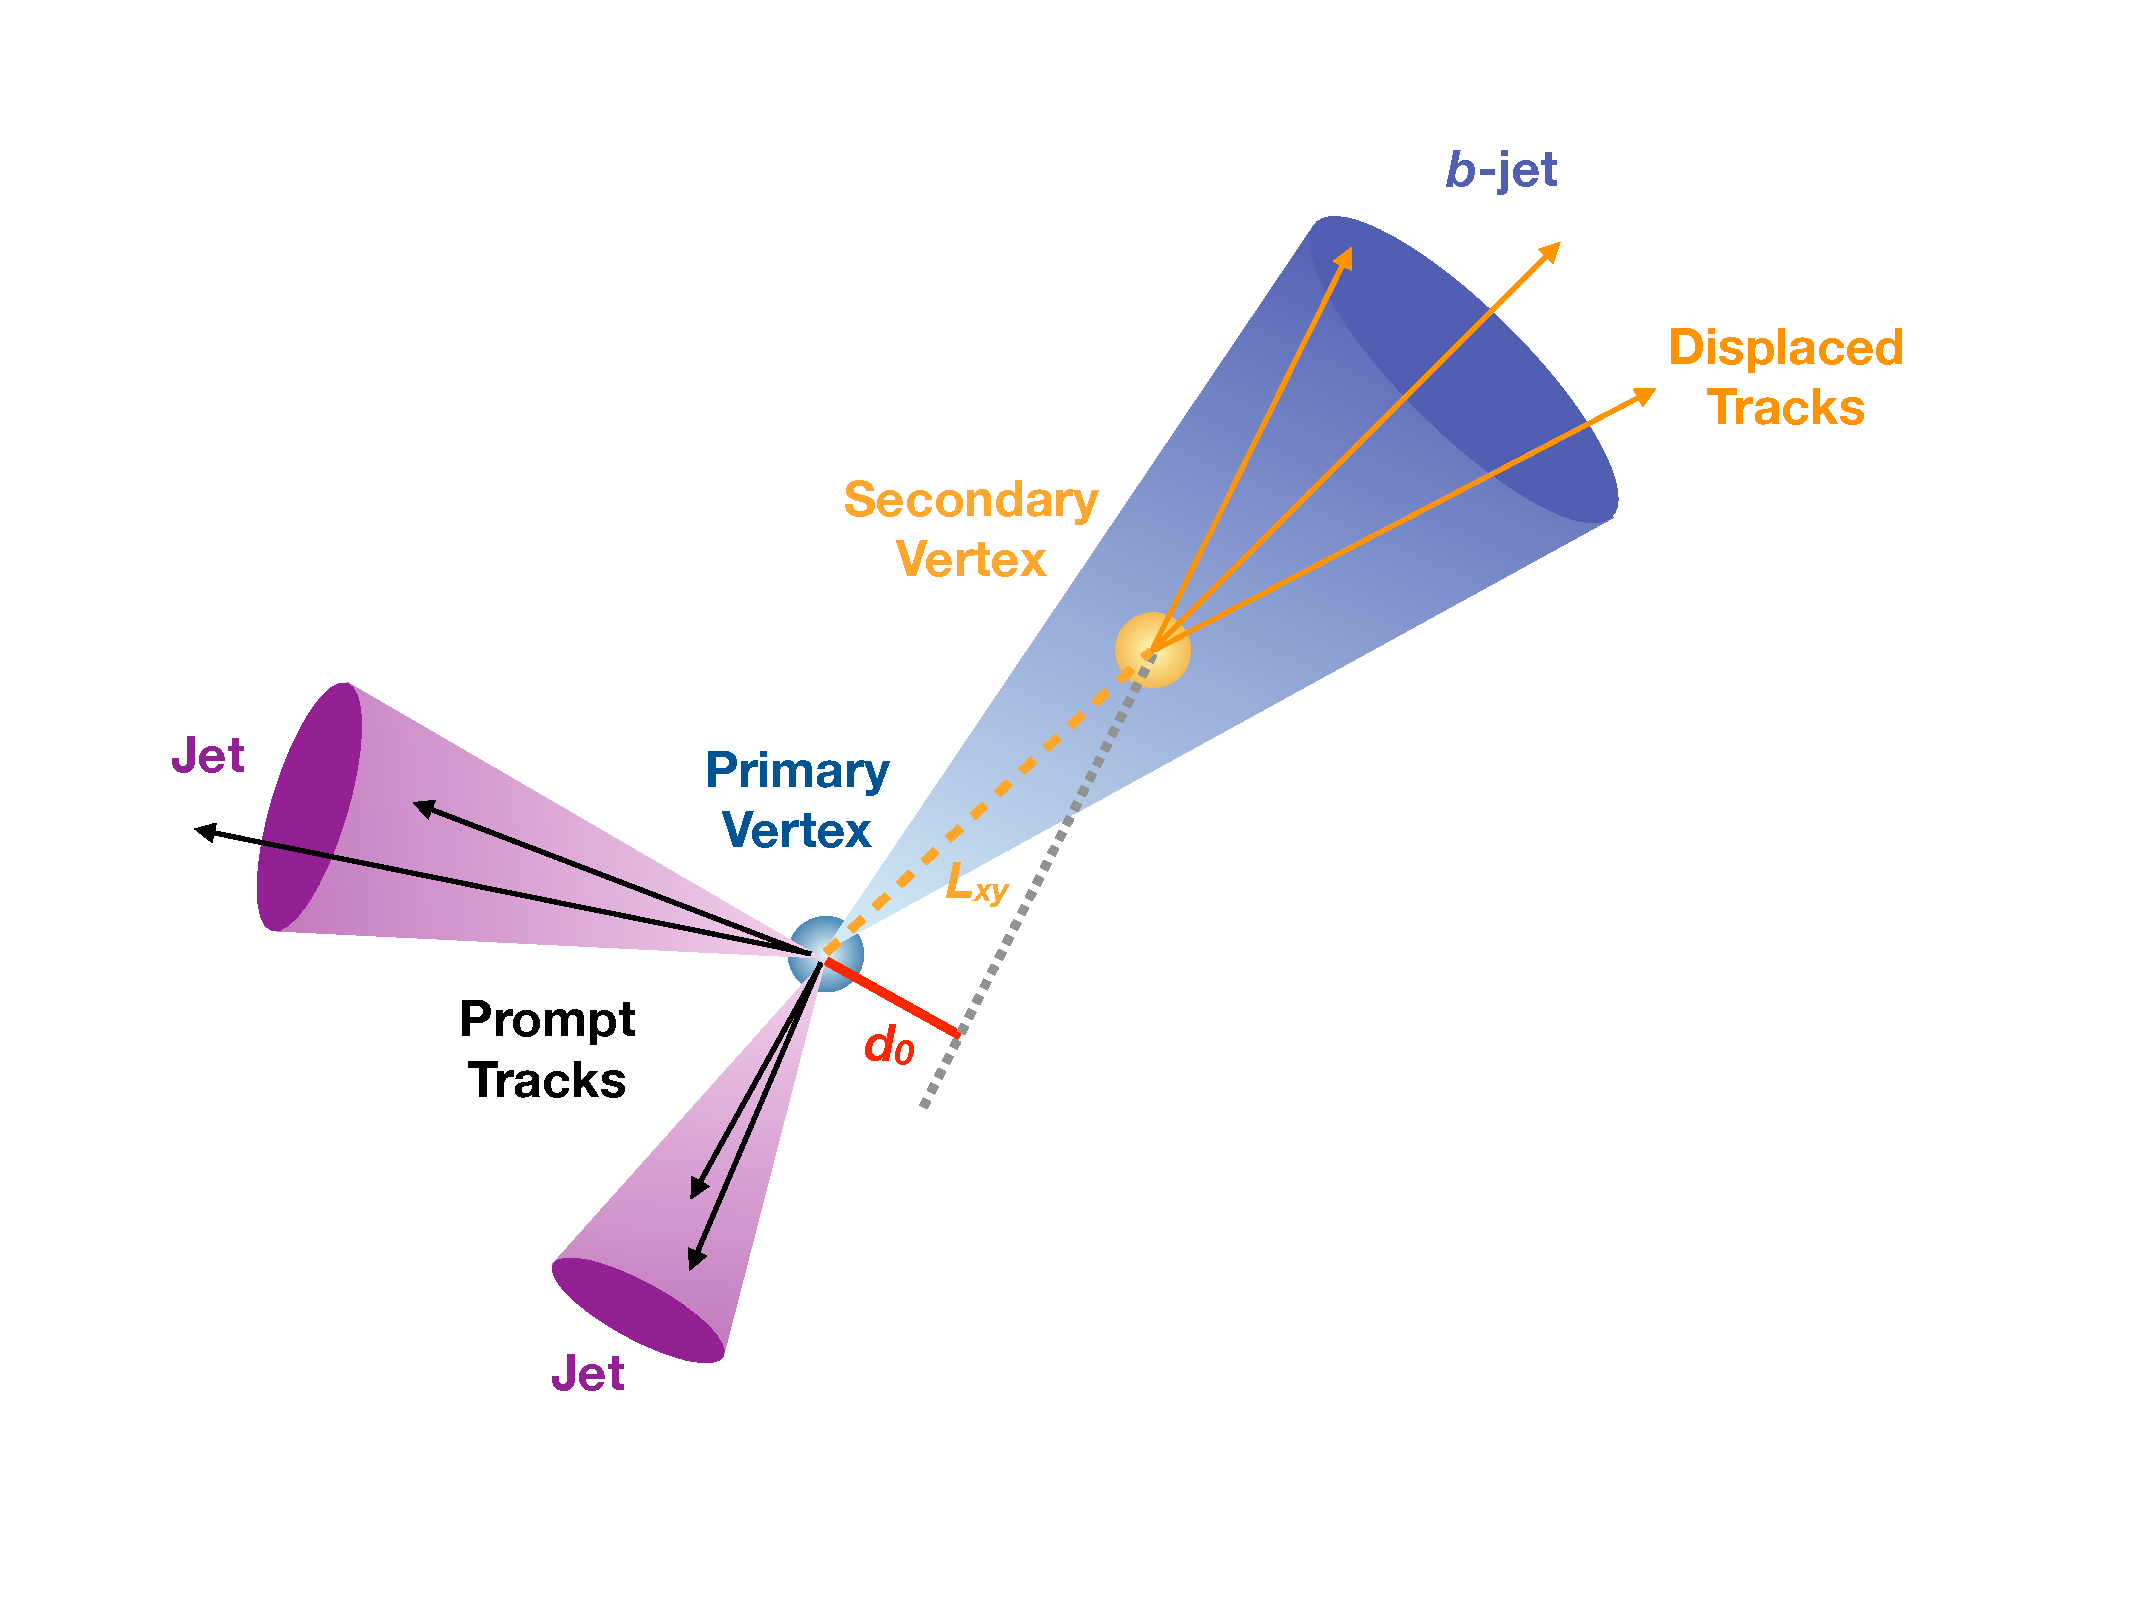
\includegraphics[width=0.8\textwidth]{figures/bjet-diagram.pdf}
\caption{Illustration of an interaction producing two light jets and one $b$-jet. While the light jets 
decay ``promptly'', coinciding with the primary vertex of the proton-proton interaction, the longer lifetime of 
$B$ hadrons leads to a secondary decay vertex, displaced from the primary vertex by length $L_{xy}$. This is 
typically a few mm, and therefore is not directly visible in the detector, but leads to a large transverse impact 
parameter, $d_{0}$, for the resulting tracks~\cite{bjettrigger}}
\end{figure}

Coming to the mass, $B$ mesons have masses of around \SI{5.2}{\GeV}, whereas the $\pi^{0}$ mass is around \SI{0.134}{\GeV},
(around 40 times lighter). This higher mass gives access to a larger decay phase space, leading to a high multiplicity 
for $b$-jets (average of 5 charged particles per decay).

One final distinguishing feature of $B$ hadrons is their \emph{fragmentation function}, a function describing the 
production of an observed final state. For $B$ hadrons, this is particularly ``hard'', with the $B$ hadrons themselves 
contributing to an average of around 75~\% of the $b$-jet energy. Thus, the identification of $b$-jets with $B$ hadrons 
is, in some sense, descriptive.

We have contrasted $b$-jets and light jets, demonstrating that there are several handles available for making this 
distinction. $c$-jets are slightly more similar to $b$-jets, but the same handles still apply -- $c$-hadron lifetimes are
between \SIlist{0.5;1}{\ps}, a factor of 2 smaller than $B$ hadrons. Their mass is around \SI{1.9}{\GeV}, 2 to 3 times 
smaller than $B$ hadrons, and $c$-hadrons contribute to an average of around 55~\% of $c$-jet energy. Therefore, while 
the gap is slightly smaller, a distinction may still be made.

The ATLAS flavor tagging framework~\cite{FTAG-2018-01} relies on developing a suite of low level taggers and 
aggregating the results of these low level taggers into a high level discriminant. We discuss each component of 
this in the following.





